\documentclass[12pt,letterpaper]{article}
\usepackage[utf8]{inputenc}
\usepackage{amsmath,amsthm,amsfonts,amssymb,amscd}
\usepackage[table]{xcolor}
\usepackage[margin=2.5cm]{geometry}
\usepackage{ragged2e}
\usepackage{graphicx}
\usepackage{multicol}
\newlength{\tabcont}
\setlength{\parindent}{0.0in}
\setlength{\parskip}{0.05in}

\begin{document}

    \textbf{Nome}: Luís Felipe de Melo Costa Silva \\
    \textbf{Número USP}: 9297961 
        
    \begin{center}
        \LARGE \bf
        Lista de Exercícios 1 - MAC0315
    \end{center}

    \section{Exercícios sobre modelagem}

    \subsection{} Com os dados apresentados, fiz uma tabela:
    
    \begin{center}
	    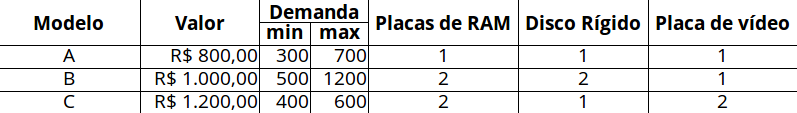
\includegraphics[width=13cm]{1-1.png}
    \end{center}
    
    A empresa possui 3000 placas de RAM, 2500 discos rígidos e 2250 placas de vídeo.
    
    Definindo como $x$ a quantidade de modelos A a serem produzidos, como $y$ a de modelos B e como $z$ a de modelos C ($x,y,z \in \mathbb{Z}$), teremos o seguinte programa linear:
    
    \begin{alignat*}{2}
	    \text{max  } & u = 800x+1000y+1200z  \\
	    \text{suj  } & 300 \leq x \leq 700\\
	                 & 500 \leq y \leq 1200\\
	                 & 400 \leq z \leq 600\\
	                 & x+2y+2z \leq 3000\\
	                 & x+2y+z \leq 2500\\
	                 & x+y+2z \leq 2250\\
    \end{alignat*}
	
	onde $u$ é o lucro, que queremos maximizar.
	
	\subsection{ } Vamos definir como $x_i$ a variável que indica se a antena $i$ foi instalada, onde:
	
	\begin{equation}
		x_i=
		\begin{cases}
			1, & \text{se a antena $i$ foi instalada} \\
			0, & \text{c.c.}
		\end{cases}
	\end{equation}
	
	Então, teremos o seguinte programa linear:
	
	\begin{alignat*}{2}
		\text{min  } & u = \sum_{i=1}^{n} x_ic_i \\
		\text{suj  } & \sum_{i=1}^{n} x_i : x_i \text{ atende a região $1$} \geq 1\\
			         & \vdots \\
		             & \sum_{i=1}^{n} x_i : x_i \text{ atende a região $m$} \geq 1\\
	\end{alignat*}
	
	onde $u$ é o custo, que queremos minimizar.
	
	\subsection{ } Definindo como $x_{ij}$ a váriavel que indica se o caixeiro-viajante foi da cidade $i$ direto para a cidade $j$, onde:
	
	\begin{equation}
		x_{ij}=
		\begin{cases}
			1, & \text{o caminho vai da cidade $i$ para a cidade $j$} \\
			0, & \text{c.c.}
		\end{cases}
	\end{equation}
	
	O modelo de programação linear usado para a resolução será:
		
	\begin{alignat*}{2}
		\text{min  } & u = \sum_{i=1}^{n} \sum_{j=1, j\neq i}^{n} x_{ij}c_{ij} \\
		\text{suj  } & \sum_{i=1, i \neq j}^{n} x_{ij} = 1 &,j = 1,...,n\\
		             & \sum_{j=1, j \neq i}^{n} x_{ij} = 1 &,i = 1,...,n\\
		             & u_i - u_j + nx_{ij} \leq n-1        &,2\leq i\neq j \leq n
	\end{alignat*}
	
	Queremos minimizar o custo $u$. As primeiras duas restrições são para garantir que apenas um caminho sai de cada cidade, e apenas um entra na cidade. A última é para garantir que teremos apenas 1 caminho ligando as cidades, e não 2 ou mais caminhos disjuntos fazendo isso, com o uso das variáveis $u_i \in \mathbb{Z}$.
	
	\subsection{ } No período dos $n$ meses, para cada período $t$, nós queremos minimizar o custo de produção $u$, que será dado por:
	
	 \begin{alignat*}{2}
		 \text{max  } & u =f_t+(p_t+h_t)\cdot (\sum_{i}^{n} x_i)  \\
		 \text{suj  } & \sum_{i}^{n} x_i \leq d_t\\
		              & \sum_{i}^{n} x_i \leq M_t\\
	 \end{alignat*}
	 
	 onde $x_i$ é a variável que representa quantas unidades foram produzidas no mês $i$.
	 
	 \section{Exercícios sobre a estrutura de programação linear}
	 
	 \subsection{ }
	 
	 Vamos aplicar a definição de conjunto convexo aqui, que é:
	 
	 \begin{center}
	 	$A \subseteq \mathbb{R}^n$ é convexo se $x,y \in A \implies \alpha x+(1-\alpha)y \in A$
	 \end{center}
	 
	 Se $a^Tx \geq b$, então $\alpha a^Tx \geq \alpha b \text{ (I)}, \forall \alpha \in [0,1]$.\\ Seja $y \in \mathbb{R}^n$. Se $a^Ty \geq b$, então $\alpha a^Ty \geq \alpha b, \text{e também } (1-\alpha) a^Ty \geq (1-\alpha) b\text{, (II) } \forall \alpha \in [0,1].$
	 
	 Somando as duas retas, temos que $\alpha a^Tx + (1-\alpha)a^Ty \geq b $, que mostra que o conjunto viável é convexo.
	 
	 \subsection{ }
	 
	 Seja $S_i$ um conjunto convexo para $i=1,...,n$. Para todo $x,y \in \bigcap_{i=1}^n S_i$ e um $\alpha \in [0,1]$ implica que $\alpha x + (1-\alpha)y \in S_i$, já que $S_i$ é convexo. Portanto, $\alpha x + (1-\alpha)y \in \bigcap_{i=1}^n S_i$, e então, $\bigcap_{i=1}^n S_i$ é convexo.
	 
	 \subsection{ }
	
	 \subsection{ }
	 
	 Na forma canônica, o programa fica assim (omitindo $x_4$, $x_5$ e $x_6$ pois não estão na função objetiva e não interferem no resultado e trocando $x_1$ por $x$, $x_2$ por $y$ e $x_3$ por $z$, por conveniência):
	 
	 \begin{alignat*}{2}
	 \text{max  } & u = 10x+12y+12z  \\
	 \text{suj  } & x+2y+2z -20 = -r\\
				  & 2x+y+2z -20 = -s\\
				  & 2x+2y+z -20 = -t\\
				  & x,y,z \geq 0\\
	 \end{alignat*}
	 
	 Seguem os tableaux:
	 
	 \begin{center}
	 	 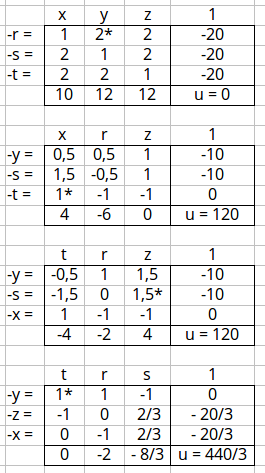
\includegraphics{3-1.png}
	 \end{center}
	 
	 
\end{document}